\documentclass[border=10pt]{standalone}
\usepackage{tikz}
\usetikzlibrary{arrows.meta, positioning, calc}
\usepackage[dvipsnames]{xcolor}

\definecolor{c1}{HTML}{4A6FA5}
\definecolor{c2}{HTML}{5B8DB8}
\definecolor{c3}{HTML}{47967A}
\definecolor{c4}{HTML}{3A9B8C}
\definecolor{c5}{HTML}{E8973A}
\definecolor{c6}{HTML}{D4764E}
\definecolor{c7}{HTML}{C05A5A}

\begin{document}

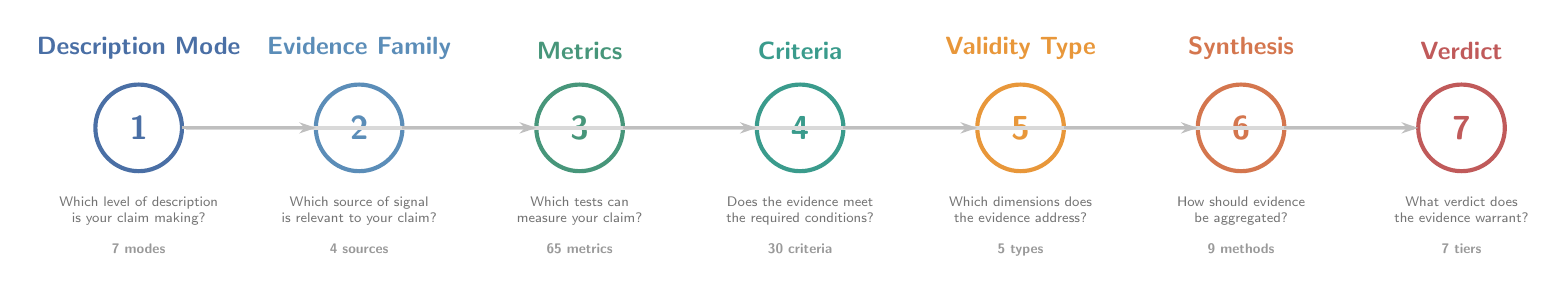
\begin{tikzpicture}[
    arr/.style={-{Stealth[length=6pt, width=4pt]}, line width=1pt, black!25},
]

% === NODES (circles with numbers) ===
\foreach \i/\col/\num/\name/\desc/\count [count=\idx] in {
    0/c1/1/Description Mode/Which level of description\\is your claim making?/7 modes,
    2.8/c2/2/Evidence Family/Which source of signal\\is relevant to your claim?/4 sources,
    5.6/c3/3/Metrics/Which tests can\\measure your claim?/65 metrics,
    8.4/c4/4/Criteria/Does the evidence meet\\the required conditions?/30 criteria,
    11.2/c5/5/Validity Type/Which dimensions does\\the evidence address?/5 types,
    14.0/c6/6/Synthesis/How should evidence\\be aggregated?/9 methods,
    16.8/c7/7/Verdict/What verdict does\\the evidence warrant?/7 tiers%
}{
    % Circle
    \draw[\col, line width=1.5pt] (\i, 0) circle (0.55cm);
    \node[font=\sffamily\large\bfseries, \col] at (\i, 0) {\num};
    % Title above
    \node[font=\sffamily\small\bfseries, anchor=south, \col] at (\i, 0.75) {\name};
    % Description below
    \node[font=\sffamily\tiny, anchor=north, align=center, text=black!55] at (\i, -0.75) {\desc};
    % Count at bottom
    \node[font=\sffamily\tiny\bfseries, anchor=north, text=black!40] at (\i, -1.35) {\count};
}

% === CONNECTING LINE ===
\draw[black!15, line width=1.5pt] (0.6, 0) -- (16.2, 0);

% === ARROWS between circles ===
\foreach \a/\b in {0.55/2.25, 3.35/5.05, 6.15/7.85, 8.95/10.65, 11.75/13.45, 14.55/16.25}{
    \draw[arr] (\a, 0) -- (\b, 0);
}


\end{tikzpicture}

\end{document}
